\documentclass[border=10pt]{standalone}
\usepackage[svgnames]{xcolor}
\usepackage{amsmath}
\usepackage{pgfplots}
\pgfplotsset{compat=newest}
\usepackage[sfdefault]{FiraSans}
\usepackage{FiraMono}
\renewcommand*\familydefault{\sfdefault}
\begin{document}
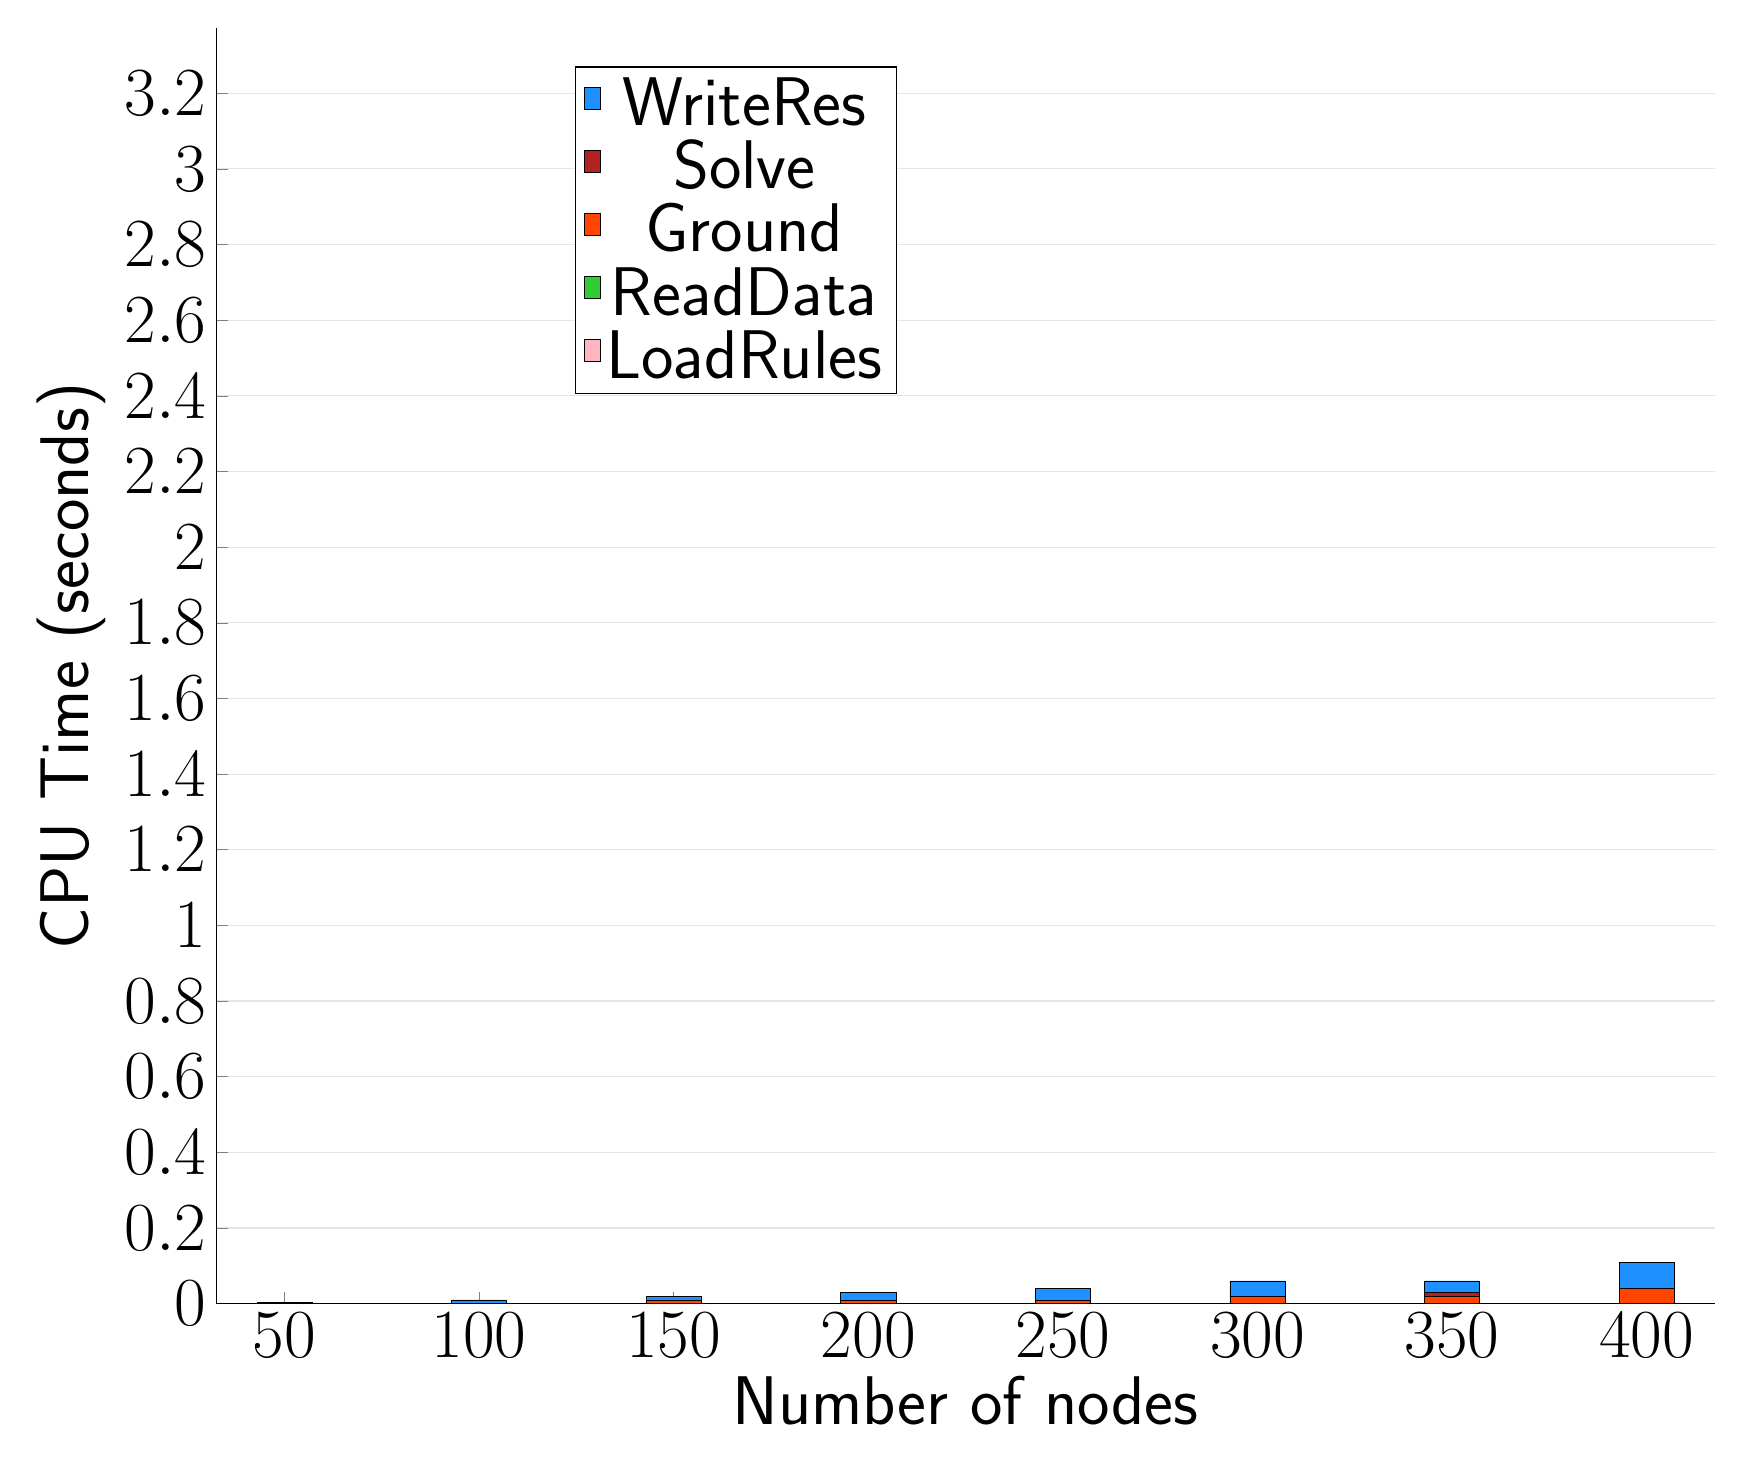
\begin{tikzpicture}
\begin{axis}[
   ybar stacked,
   width=1.7\textwidth,
   bar width=0.7cm,
   ymajorgrids, tick align=inside,
   major grid style={draw=gray!20},
   xtick=data,
   ymin=0, ymax=3.3720000000000003,
   axis x line*=bottom,
   axis y line*=left,
   enlarge x limits=0.05,
   legend style={
       at={(0.454, 0.97)},
       anchor=north east,
       legend columns=1,
       font=\Huge,
   },
   ylabel={CPU Time (seconds)},
   xlabel={Number of nodes},
   label style={font=\Huge},
   tick label style={font=\Huge},
]
\addlegendimage{fill=DodgerBlue, draw=black, line width=0.2pt}
\addlegendentry{WriteRes}
\addlegendimage{fill=FireBrick, draw=black, line width=0.2pt}
\addlegendentry{Solve}
\addlegendimage{fill=OrangeRed, draw=black, line width=0.2pt}
\addlegendentry{Ground}
\addlegendimage{fill=LimeGreen, draw=black, line width=0.2pt}
\addlegendentry{ReadData}
\addlegendimage{fill=LightPink, draw=black, line width=0.2pt}
\addlegendentry{LoadRules}
\addplot +[fill=LightPink, draw=black, line width=0.2pt] coordinates {
(50, 0.0)
(100, 0.0)
(150, 0.0)
(200, 0.0)
(250, 0.0)
(300, 0.0)
(350, 0.0)
(400, 0.0)
};
\addplot +[fill=LimeGreen, draw=black, line width=0.2pt] coordinates {
(50, 0.0)
(100, 0.0)
(150, 0.0009999999999999998)
(200, 0.0)
(250, 0.0)
(300, 0.0)
(350, 0.0)
(400, 0.0)
};
\addplot +[fill=OrangeRed, draw=black, line width=0.2pt] coordinates {
(50, 0.0009999999999999998)
(100, 0.0)
(150, 0.008999999999999998)
(200, 0.009999999999999997)
(250, 0.009999999999999997)
(300, 0.019999999999999997)
(350, 0.019999999999999997)
(400, 0.03999999999999999)
};
\addplot +[fill=FireBrick, draw=black, line width=0.2pt] coordinates {
(50, 0.0)
(100, 0.0)
(150, 0.0)
(200, 0.0)
(250, 0.0)
(300, 0.0)
(350, 0.010000000000000004)
(400, 0.0)
};
\addplot +[fill=DodgerBlue, draw=black, line width=0.2pt] coordinates {
(50, 0.0029999999999999996)
(100, 0.009999999999999997)
(150, 0.010000000000000004)
(200, 0.020000000000000007)
(250, 0.030000000000000006)
(300, 0.039999999999999994)
(350, 0.029999999999999992)
(400, 0.07000000000000002)
};
\end{axis}
\end{tikzpicture}

\end{document}
